\documentclass{article}

\usepackage{fancyhdr}
\usepackage{hyperref}
\usepackage{pageslts}
\usepackage{graphicx}
\usepackage{amsmath}
\usepackage{amssymb}

\newcommand{\chili}{
\includegraphics[height=1ex]{chili}}

\lhead{Jason Gross}
\chead{Mathcamp Mentor Application}
\rhead{\today}
\cfoot{\thepage\space of \lastpageref{LastPage}}
\pagestyle{fancy}

\begin{document}
\pagenumbering{arabic}

% READY TO APPLY?
%
% Write us a page or two about yourself, why you want to join Mathcamp and how you think you could contribute. Describe your qualifications, experience (construe that broadly), ideas, etc.


%
% Describe, in a half-page to a page, a class or independent student project that you would like to run at Mathcamp. Feel free to design your dream class or ideal project. Make sure to include some details, like difficulty, pacing, problems you might assign, etc. Keep in mind that these are bright high school students who can accomplish a lot -- but have limited time, and varying mathematical backgrounds. Some of them may meet modular arithmetic for the very first time at camp (but will be quick to pick it up and run with it); a few will have already taken classes at college, and will happily follow a development of Stokes' Theorem on manifolds; most fall somewhere in between. What we are most looking for is a coherent, interesting curriculum that demonstrates your creativity as a teacher.
%
% In addition to your detailed class proposal, please give several brief descriptions (a sentence or two is fine) for 2-3 other classes or projects that you might like to run at Mathcamp. Please include enough details for us to understand the content of the course and the main ideas that students should take away; we would like to see your breadth as a teacher and your range as a mathematician.
%
% We'd also like to hear any new ideas you have for interesting and fun activities, whether they are math-related or not.
%
% We want to get an overall feeling for who you are, and how you would fit into our community, but your application needn't be longer than a few pages. Include your name, year, school, mathematical and teaching interests, and the best way for us to contact you. Please email your application (either as a PDF, or as plain text in the body of your e-mail), along with a CV, to David Savitt <savitt@mathcamp.org> by February 24, 2014.
%
% IN ADDITION...
%
% We also ask for one letter of recommendation on your behalf. We are interested in both your mathematical strength and in your teaching experience and expertise. (It is worth stressing that some of our best mentors have had little formal teaching experience before their first summer at Mathcamp.) Though it is by no means a requirement, you may submit two recommendation letters: one from someone who knows you well mathematically, and one from someone who is familiar with your teaching ability. In any case, please show our description of the mentor position to your recommender, and ask your recommender to comment on your suitability for such a job.
%
% Again we ask that the recommendation letter be sent to us via email, that it either be a PDF or plain text, and that we receive the letter on or before February 24, 2014. (We will begin reviewing applications promptly after the deadline.)
%
% Also, if you know someone who has been involved in Mathcamp in the past, and you would like us to keep them in mind as a reference, please include their name and email address.
%
% When we receive your application, we will send you an acknowledgment; if you have not heard from us, please feel free to write to us to confirm the receipt of your application. We plan to make our first round of offers by March 17.
%
% Note: We ask staff to arrive by July 2 and leave August 14. (The campers arrive on July 6 and depart on August 10.) However, if you can only make it for (a significant) part of that time, please get in touch with us anyway.
%
% Thanks very much for your interest in Mathcamp!
%
%
% David Savitt
% Jan 28 (3 days ago)
%
% TEACHING COMPUTER SCIENCE AT MATHCAMP:
%
% Every year we try to include several computer science classes. In the past topics have included cryptography, quantum computing, and computational complexity theory. These classes are often very popular with the students and so we are very excited to have applicants who are interested and able to teach them. Sometimes these classes are taught by math graduate students with an interest in CS, but in the past we have also had mentors who are computer science students with a strong interest in mathematics.


\subsubsection*{About Me}
% Write us a page or two about yourself, why you want to join Mathcamp and how you think you could contribute. Describe your qualifications, experience (construe that broadly), ideas, etc.
{\setlength{\parindent}{0pt}
\setlength{\parskip}{0.5\baselineskip}
I'm a first year grad student in computer science, working with Adam Chlipala at MIT on verified program synthesis (making verified compilers smart enough to perform algorithm-level optimizations on code based on mathematical descriptions), and separately on formalizing category theory in the proof assistant Coq on top of homotopy type theory.  As an undergrad, also at MIT, I majored in mathematics and computer science, with a humanities concentration in philosophy.  The four summers prior to my undergraduate career, I attended Mathcamp.  Those summers were the best twenty weeks of my life up to that point, and probably still rate as the best summers I've ever had.  I loved the math, the people, and the community.  I want to be a part of that environment again, and contribute more to it.

The role of being a mentor appeals to me because I enjoy teaching and helping people understand things better.  My friends tell me that I'm very good at explaining concepts.  I love learning, and enjoy learning from my students.  As an undergrad, I was a teaching assistant for introductory physics for three years in MIT's Experimental Study Group (ESG); I held office hours to help students better understand concepts and solve pset problems, and I once gave a lecture on the principle of least action.  In feedback, students gave me high ratings, praising my dedication, patience, and understanding, both of them and the mathematics and physics.  They liked that I didn't just give them the answers, and instead helped them discover things for themselves.

When I present a topic, and a student doesn't understand it, I then need to figure out why.  I try to understand how the student is approaching the topic, and what the student's current conception is.  The process of bridging the gap between my understanding and the student's, and the process of helping the student to pinpoint the gap and traverse it, often leaves me with a better understanding of the material.  For this reason, among others, I've been teaching classes every year for MIT's Educational Studies Program (ESP) for Splash, Spark, and HSSP; the topics have included category theory, linear logic, homotopy type theory, sizes of infinity, ordinal arithmetic, philosophy, quantum mechanics, \LaTeX, computer-assisted theorem proving, and linear algebra.

Finally, math is beautiful.  I want to share that beauty with others, and appreciate it with them.  Most recently, I've been involved in the new and exciting field of homotopy type theory, which promises to provide an alternative to set theory for founding formal mathematics in a way which allows informal math to be much closer to formal mathematics.  Although it was founded around 2006-2009, homotopy type theory only really got going at the IAS 2012-2013, and I want to share the excitement of being in a new field of math with others.

In summary, I believe that I can share interesting, beautiful, and exciting math and computer science with campers, and that I have the skills and motivation to be an engaging and compassionate mentor.
}
\clearpage
\subsubsection*{Class: Exploring equality via homotopy and proof assistants\texorpdfstring{ (\chili\chili\,--\chili\chili\chili)}{}}
%- Class description (0.5--1 pages)
%  - Prompt
%    - Describe, in a half-page to a page, a class or independent student project that you would like to run at Mathcamp. Feel free to design your dream class or ideal project. Make sure to include some details, like difficulty, pacing, problems you might assign, etc. Keep in mind that these are bright high school students who can accomplish a lot -- but have limited time, and varying mathematical backgrounds. Some of them may meet modular arithmetic for the very first time at camp (but will be quick to pick it up and run with it); a few will have already taken classes at college, and will happily follow a development of Stokes' Theorem on manifolds; most fall somewhere in between. What we are most looking for is a coherent, interesting curriculum that demonstrates your creativity as a teacher.
\noindent \textbf{Blurb}: What does it mean for two things to be equal?  What if the things are themselves proofs of equality?  Homotopy type theory, and exciting new branch of mathematics which could replace set theory as the foundation of mathematics, has recently provided a new way of looking at proofs equality as paths in a topological space.  In this class, we will explore the nature of equality using Coq, an interactive theorem prover.

\noindent\textbf{Prerequisites}: Proof by induction, formal logic.  Optionally, programming.

\noindent\textbf{Syllabus Outline}:

\begin{itemize}
  \item
    Guided discussion --- How do we use equality?  What properties should equality have?  What properties should it not have?
    \begin{itemize}
      \item reflexivity, symmetry, transitivity (equivalence relations)
        %- but not for NaN in floating point in computers
        %  - This was probably a mistake, but shows that it's something we have to think about
      %- symmetry
      %- transitivity
      %  - sometimes; what about approximately equal?
      \item substitution
        %- Except +0 = -0, but +inf != -inf in floating point
      \item isomorphism
      \item How do we prove equality?
      \begin{itemize}
        \item by transitivity% (each equal to something we already know)
        , symmetry, reflexivity
        %- by symmetry
        %- by reflexivity
        \item by computation rules, or other axioms, maybe with substitution ($n + n = 2 \times n$; or $2 \times 3 = 6$)
        \item by induction (e.g., on natural numbers, showing $+$ commutes)
        \item by functional extensionality ($(\forall x, f(x) = g(x)) \to f = g$)
      \end{itemize}
      \item What do we do with proofs of equality?  (One answer: substitution)
      \item Parting question: When are two proofs of equality the same? (e.g., proof that $x + y = y + x$ by induction on $x$ then on $y$, vs.~on $y$ then on $x$, vs.~first apply symmetry then do double induction)
      \item Homework
      \begin{itemize}
        \item Think about when proofs of equality are the same, try to prove things in two ways related ways, and see if you can prove that the proofs are equal.
        \begin{itemize}
          \item $\forall x\ y, x + y = y + x$
          \item $\forall x\ y\ z, (x + y) + z = x + (y + z)$
        \end{itemize}
        \item Stare at J rule \\
          (\texttt{$\forall$~(A~:~Type) (x~:~A) (P~:~$\forall$ y, x = y $\to$ Type), \\ P x refl $\to$ $\forall$~y (H~:~x = y), P y H}) \\
          and K rule \\
          (\texttt{$\forall$~(A~:~Type) (x~:~A) (P~:~x = x $\to$ Type), \\ P refl $\to$ $\forall$~(H~:~x~=~x), P H}), \\
          say what they mean in words
      \end{itemize}
    \end{itemize}
    \item Exploring the J rule and the K rule in a proof assistant
    \begin{itemize}
      \item Introduce Coq, how to prove things by induction (lecture and demo)
      \begin{itemize}
        \item simplification by computation
        \item reflexivity of equality
        \item induction on natural numbers to prove addition is commutative, associative (students attempt themselves)
      \end{itemize}
      \item Introduce definition of equality in Coq (lecture)
      \begin{itemize}
        \item explain syntactic equality, computation
      \end{itemize}
      \item eliminator (J rule) (in-class exercises)
      \begin{itemize}
        \item prove symmetry, transitivity
        \item Prove \texttt{sym (sym p) = p}
        \item Prove \texttt{trans refl p = p}
        \item Prove \texttt{trans p refl = p}
      \end{itemize}
      \item Homework
      \begin{itemize}
        \item Prove UIP (uniqueness of identity proofs, \texttt{$\forall$ A (x~:~A) (p q~:~x = x), p = q}) from K
        \item Explore what else you can prove about equality in general.
        \begin{itemize}
          \item Can you prove K (or UIP) from J?
          \item relation between \texttt{sym} and \texttt{trans}?
          \item how many proofs of symmetry are there? (up to equality?)
          \item \ldots\space of transitivity?
          \item can you relate proof of \texttt{sym (sym p) = p} to other things?
        \end{itemize}
      \end{itemize}
    \end{itemize}
    \item Univalence --- isomorphism (equivalence) and equality
    \begin{itemize}
      \item Define equivalence ($\simeq$) for students (by bi-invertible map: $f : A \to B$ is an equivalence if we have $g, h : B \to A$ and $g \circ f = 1$ and $f \circ h = 1$)
      \item Proofs about equivalence (student-guided)
      \begin{itemize}
        \item all proofs that $f$ is an equivalence are equal
        \item implies quasi-inverse ($g$ such that $f \circ g = 1$ and $g \circ f = 1$, with no relation between the proofs)
        \item reflexivity
        \item symmetry
        \item transitivity
      \end{itemize}
      \item Describe univalence (\texttt{idtoequiv}$ : x = y \to x \simeq y$ is an equivalence)
      \begin{itemize}
        \item how many proofs are there of bool = bool?
      \end{itemize}
    \end{itemize}
    \item Inductive types and their equalities (possibly lecture, or possibly guided exploration individually or in small groups)
    \begin{itemize}
      \item decidable equality $\to$ UIP
      \begin{itemize}
        \item natural numbers
        \item booleans
      \end{itemize}
      \item pattern matching and induction as fundamental
      \item disjoint union/sum types
      \item cartesian product/sigma types
      \item function types/pi types
      \item classify equalities up to equivalence
      \item interesting puzzle (homework problem?): The type \texttt{\{ x : A | y = x \}} is contractible (it has an inhabitant, and all inhabitants are provably equal), even though the type \texttt{x = x} isn't.  But equals are interchangeable, so why aren't all proofs of \texttt{x = x} equal?
    \end{itemize}
    \item Higher inductive types --- custom equalities
    \begin{itemize}
      \item Define the interval (two points and a path (proof of equality) between them)
      \begin{itemize}
        \item Challenge: prove functional extensionality from the interval
      \end{itemize}
      \item Define truncation
      \item Define the circle
      \begin{itemize}
        \item Challenge: prove that the truncation of the type \texttt{base = base} is isomorphic to the integers (i.e., $\pi_1(S^1) \simeq \mathbb{Z}$)
      \end{itemize}
      \item Further exploration: truncation types, homotopies, axioms of choice, laws of excluded middle
  \end{itemize}
\end{itemize}
\clearpage
\subsubsection*{Other ideas for classes and projects}
% In addition to your detailed class proposal, please give several brief descriptions (a sentence or two is fine) for 2-3 other classes or projects that you might like to run at Mathcamp. Please include enough details for us to understand the content of the course and the main ideas that students should take away; we would like to see your breadth as a teacher and your range as a mathematician.
\begin{itemize}
  \item
    Incompleteness theorems --- G\"odel's incompleteness theorem, the halting problem, L\"ob's theorem, diagonalization arguments
  \item
    Exploring Noether's theorem through parametricity and programming languages --- Noether's theorem is a very general and beautiful result in theoretical physics that relates differentiable symmetries to conserved quantities.  Parametricity is the property that programs are invariant under changes of data representation; it allows you to derive ``theorems for free'', such as that the only (computable) function of type $\forall X, X \to X$ is the identity function.  A recently published paper%\footnote{Robert Atkey. From Parametricity to Conservation Laws, via Noether's Theorem. In \emph{Proceedings of the 41st ACM SIGPLAN-SIGACT Symposium on Principles of Programming Languages (POPL 2014)}. 2014.}
    relates these two ideas, allowing automatic derivation of conserved quantities from appropriate descriptions of physical systems.  %This could be a class on the mathematics behind these ideas, or, depending on the background, interest, and motivation of students, a project on understanding the published paper, or pushing the ideas further.
  %\item Design your own type-theory-based proof assistant --- Proof assistants allow computers to check your proofs, and allow exploration of theorems and definitions with a guide to ensure that you don't break any rules unintentionally.  %As computers get faster, these programs have gradually become more popular, showing up in more undergraduate classes and research papers.  
  %The idea, for students familiar with programming, would be to learn about how such programs work in theory and how type theory provides an alternative to axiomatic logic, by designing, and possibly implementing, a basic proof checker.
  %\item Introductory category theory --- I enjoyed Dan Zaharapol's Day Zero ``Sets, Maps, Limits, and Colimits'' class in 2009, and Noah's class on category theory through pictures.  This would be similar to one of those.
  %\item Circuits over sets of natural numbers (project originally run by Dan Zaharopol) --- Consider the following operations on sets of natural numbers: union, intersection, pointwise addition, pointwise multiplication, and set complement.  What kinds of sets can you make if you start from one-element sets?  How hard is it to decide if a number is in the set defined by a given formula?  (If you can do it in general, then you've solved Goldbach's Conjecture.)  What if you restrict which operations you're allowed to use?  (student-guided project)
  \item Prisoner's Dilemma with source code --- There is a variant of the prisoner's dilemma where each competitor receives their opponent's source code.  In this variant, it's trivial to beat the Nash equilibrium of the standard presentation, but it's highly non-trivial to figure out what ``optimal'' might mean.  This project could serve as an introduction to provability logic and model theory, in addition to game theory.
  %\item Formalizing $\langle$\emph{insert your favorite math here}$\rangle$ in a proof assistant; it turns theorem proving into a game!
  %\item Exploring homotopy type theory (probably a student-directed project)
  %\item Learn functional programming (short class, after-hours activity, or project)
  %\item Learn type theory, an alternative to axiomatic logic
  %\item Relationships between the various truncated axioms of choice and laws of excluded middle; here, truncated refers to the homotopy type of the spaces to which the axioms are restricted to. (student-directed project)
  %\item Linear logic --- In standard logic, if you have $A$, then you have $A$ and $A$.  So if you have a quarter, then you have a quarter and another quarter, right?  Linear logic is the logic of resources.
  %\item Introductory topology class, following, e.g., Munkres' \emph{Topology}
  %\item Proof techniques class, or possibly a variant of it which also introduces what a proof is, as a mathematical object.
  %\item Basic theoretical computer science --- lambda calculus, Turing machines, halting problem, computational complexity
\end{itemize}


\subsubsection*{Other fun ideas}
%- We'd also like to hear any new ideas you have for interesting and fun activities, whether they are math-related or not.
\begin{itemize}
  \item 30 constructions in 30 minutes --- like 30 proofs in 30 minutes, but rather than trying to prove things, we instead construct or define them, possibly with the necessary mathematical background definitions
  \item Indoor skydiving
  \item Trip to \href{https://maps.google.com/?ll=43.929565309931085,-124.11577032281491&q=43.929565309931085,-124.11577032281491}{sand dunes and lake} (comfortably swimmable at the end of July) (\href{https://plus.google.com/photos/103416070288920608429/albums/5905882242979530833/5905882882578571666?authkey=CNrZu8S0s6yvgQE&pid=5905882882578571666&oid=103416070288920608429}{More pictures here}, from when I went with OPLSS in summer 2013):
  \begin{center}
    \hspace{\stretch{1}}
    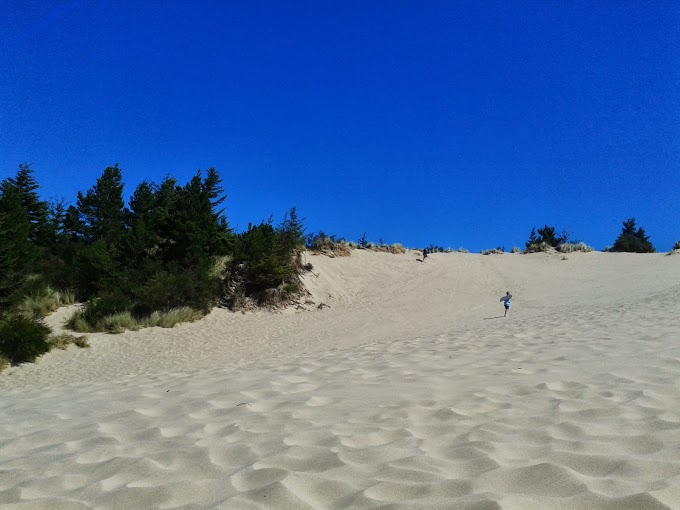
\includegraphics[width=0.45\textwidth]{2013-07-28-15-30-37.jpg}
    \hspace{\stretch{1}}
    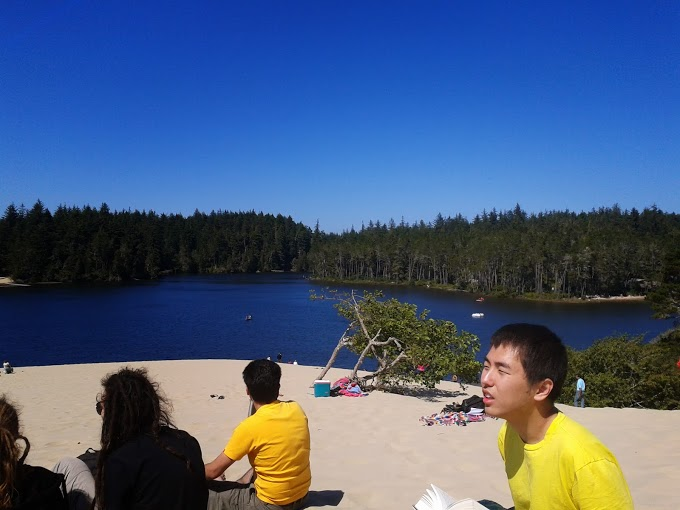
\includegraphics[width=0.45\textwidth]{2013-07-28-15-30-53.jpg}
    \hspace{\stretch{1}}
  \end{center}
  \clearpage
  \item Trip to \href{https://maps.google.com/maps?q=44.134686,-124.123456&hl=en&sll=44.032101,-124.112077&sspn=0.288791,0.676346&t=h&dirflg=w&z=16}{pretty beaches} (water is very cold at the end of July) (\href{https://plus.google.com/photos/103416070288920608429/albums/5905882242979530833/5905893435660061586?authkey=CNrZu8S0s6yvgQE&pid=5905893435660061586&oid=103416070288920608429}{More pictures here}, from when I went with OPLSS in summer 2013):
  \begin{center}
    \hspace{\stretch{1}}
    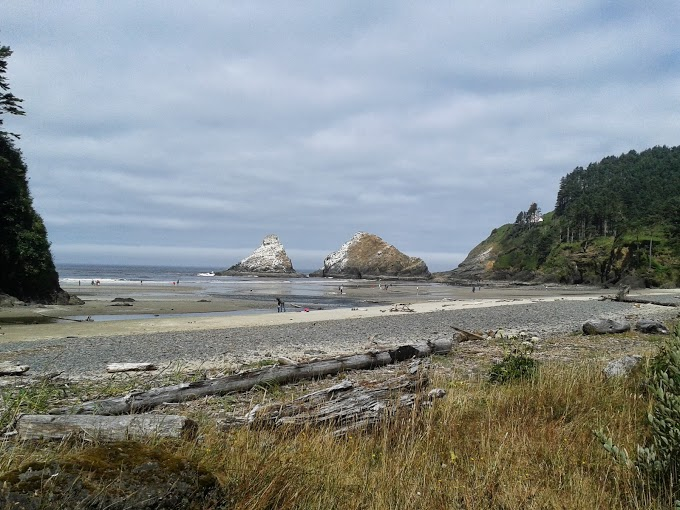
\includegraphics[width=0.45\textwidth]{2013-07-28-11-09-04.jpg}
    \hspace{\stretch{1}}
    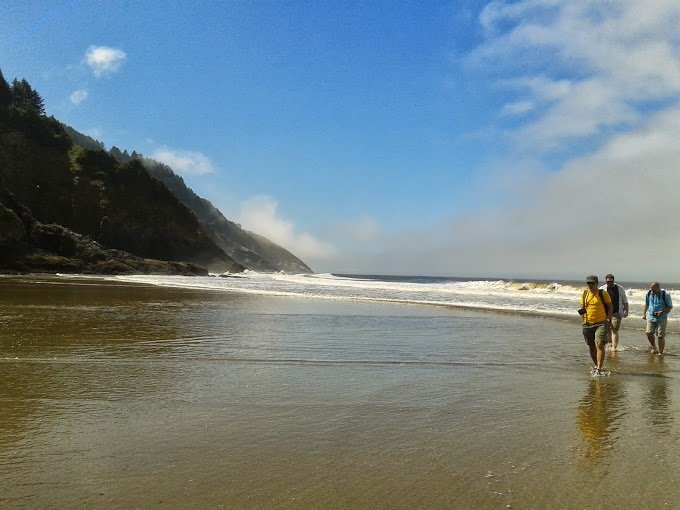
\includegraphics[width=0.45\textwidth]{2013-07-28-11-22-00.jpg}
    \hspace{\stretch{1}}
  \end{center}
\end{itemize}

\clearpage
\subsubsection*{Miscellaneous Info}
%- We want to get an overall feeling for who you are, and how you would fit into our community, but your application needn't be longer than a few pages. Include your name, year, school, mathematical and teaching interests, and the best way for us to contact you. Please email your application (either as a PDF, or as plain text in the body of your e-mail), along with a CV, to David Savitt <savitt@mathcamp.org> by February 24, 2014.
\noindent \textbf{Name}: Jason Gross \par
\noindent \textbf{School Year}: First Year PhD Student in Computer Science at MIT \par
\noindent \textbf{Contact}: \href{mailto:jasongross9@gmail.com}{jasongross9@gmail.com} (best), or %\href{tel:+16317908962}{
(631) 790-8962%}
\space (cell, second best) \par
\noindent \textbf{Mathematical and teaching interests}: Category theory, math education, foundations of math, topology, homotopy type theory, type theory, logic, proof techniques, infinity, philosophy of math, physics \par
%- We also ask for one letter of recommendation on your behalf. We are interested in both your mathematical strength and in your teaching experience and expertise. (It is worth stressing that some of our best mentors have had little formal teaching experience before their first summer at Mathcamp.) Though it is by no means a requirement, you may submit two recommendation letters: one from someone who knows you well mathematically, and one from someone who is familiar with your teaching ability. In any case, please show our description of the mentor position to your recommender, and ask your recommender to comment on your suitability for such a job.
\noindent \textbf{Reccomenders}: Peter Dourmashkin (teaching); David Spivak (math expertise) \par
%- Also, if you know someone who has been involved in Mathcamp in the past, and you would like us to keep them in mind as a reference, please include their name and email address.
\noindent Out of the people involved in Mathcamp, I think Dan Zaharopol probably knows me best personally, though Mike Shulman might know my current mathematical capabilities better, through contributions I've made to the homotopy type theory repository. \par
\noindent \textbf{Miscellaneous Concern}: I've submitted a paper to ITP 2014, which is July 14$^\text{th}$--18$^\text{th}$ in Vienna, Austria.  If the paper is accepted (I find out March 21$^\text{st}$), I may have to attend (though it's unclear if I'd have to be there for more than a day).


\end{document}